% Scattering angle versus impact parameter: hard sphere vs repulsive Coulomb.
% Hard sphere (radius a): theta = 2 arccos(b/a) for b<a, 0 otherwise.
% Coulomb V=alpha/r: theta = 2 arctan(k/b), k = alpha/(m v0^2); plotted with k=a.
% Dashed: small-angle (impulse) approximation theta = 2k/b.
% Compile: pdflatex theta_b_tikz.tex
\documentclass[tikz,border=6pt]{standalone}
\usepackage{amsmath}
\usepackage{fix-cm}
\usetikzlibrary{arrows.meta}
\begin{document}
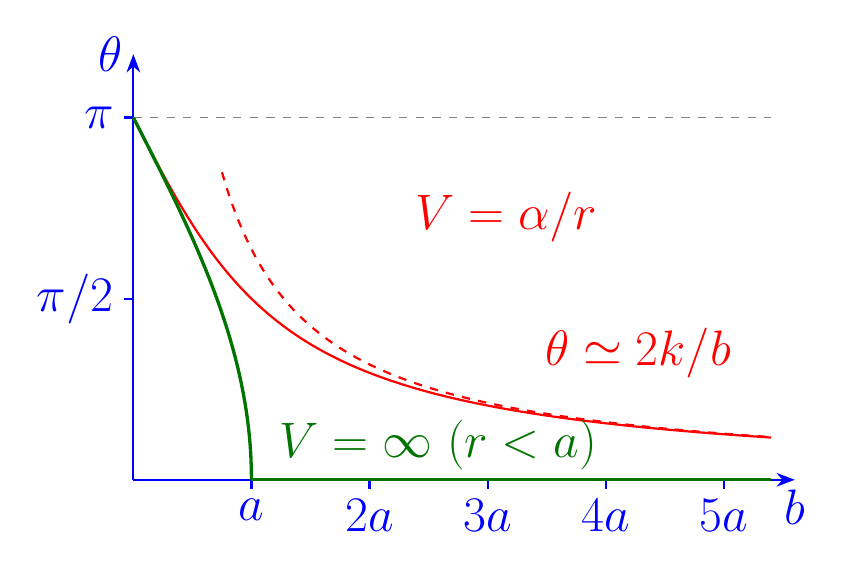
\begin{tikzpicture}[>=Stealth,thick,every node/.style={font=\fontsize{18}{22}\selectfont},
  x=1.5cm,y=1.15cm]
  % y unit: theta/(pi/4), so theta=pi is at y=4
  \draw[blue,->] (0,0) -- (5.6,0) node[below] {$b$};
  \draw[blue,->] (0,0) -- (0,4.7) node[left] {$\theta$};
  \foreach \x/\l in {1/a,2/2a,3/3a,4/4a,5/5a} {\draw[blue] (\x,0) -- (\x,-.1) node[below] {$\l$};}
  \foreach \y/\l in {2/{\pi/2},4/{\pi}} {\draw[blue] (0,\y) -- (-.08,\y) node[left] {$\l$};}
  \draw[gray,thin,dashed] (0,4) -- (5.4,4);
  % Coulomb exact
  \draw[red,domain=0.01:5.4,samples=200,smooth] plot (\x,{2*atan(1/\x)/45});
  % small-angle approximation 2k/b (radians -> y units: *4/pi)
  \draw[red,dashed,domain=0.75:5.4,samples=80,smooth] plot (\x,{(2/\x)*4/pi});
  % hard sphere
  \draw[green!45!black,very thick,domain=0:1,samples=200,smooth] plot (\x,{2*acos(\x)/45}) -- (1,0);
  \draw[green!45!black,very thick] (1,0) -- (5.4,0);
  \node[green!45!black,anchor=west] at (1.15,.38) {$V=\infty\ (r<a)$};
  \node[red,anchor=west] at (2.3,2.9) {$V=\alpha/r$};
  \node[red,anchor=west] at (3.4,1.4) {$\theta\simeq 2k/b$};
\end{tikzpicture}
\end{document}
